%%%%%%%%%%%%%%%%%%%%%%%%%%%%%%%%%%%%%%%%%%%%%%%%%%%%%%%%%%%%%%%%%%%%%%%%%%%%%%%
%optimization.tex: Detector Optimization
%%%%%%%%%%%%%%%%%%%%%%%%%%%%%%%%%%%%%%%%%%%%%%%%%%%%%%%%%%%%%%%%%%%%%%%%%%%%%%%%
\chapter{Detector Optimization}
\label{optimization_chapter}
%%%%%%%%%%%%%%%%%%%%%%%%%%%%%%%%%%%%%%%%%%%%%%%%%%%%%%%%%%%%%%%%%%%%%%%%%%%%%%%%

We optimized the detectors for a space-like environment.

%%%%%%%%%%%%%%%%%%%%%%%%%%%%%%%%%%%%%%%%%%%%%%%%%%%%%%%%%%%%%%%%%%%%%%%%%%%%%%%%
% TES Bolometer Theory {{{
%%%%%%%%%%%%%%%%%%%%%%%%%%%%%%%%%%%%%%%%%%%%%%%%%%%%%%%%%%%%%%%%%%%%%%%%%%%%%%%%
\section{Bolometer Theory}
\label{sec:tes_bolometer}
%%%%%%%%%%%%%%%%%%%%%%%%%%%%%%%%%%%%%%%%%%%%%%%%%%%%%%%%%%%%%%%%%%%%%%%%%%%%%%%%

%\textcolor{red}{Acronyms is failing us ... the figure descriptions are the first place they appear ... how do we fix this??? FIXED... BUT DON'T REMEMBER HOW :/}

\textcolor{red}{Describe how a bolometer works. Power to temperature detector.}
% Need: cartoon. }

\textcolor{red}{Figure out how to properly add Mather 1982 applied optics bolometer noise paper to bibfile and reference.}

\begin{figure}[ht!]
\begin{center}
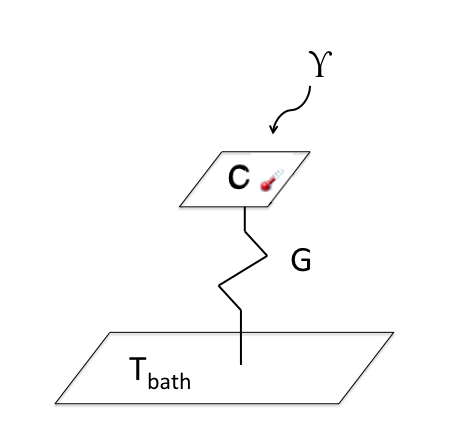
\includegraphics[height=2.5in]{figures/bolometer_cartoon}
\caption{Bolometer. 
\label{fig:bolometer_cartoon} }
\end{center}
\end{figure}


Describe TES.  
\begin{figure}[ht!]
\begin{center}
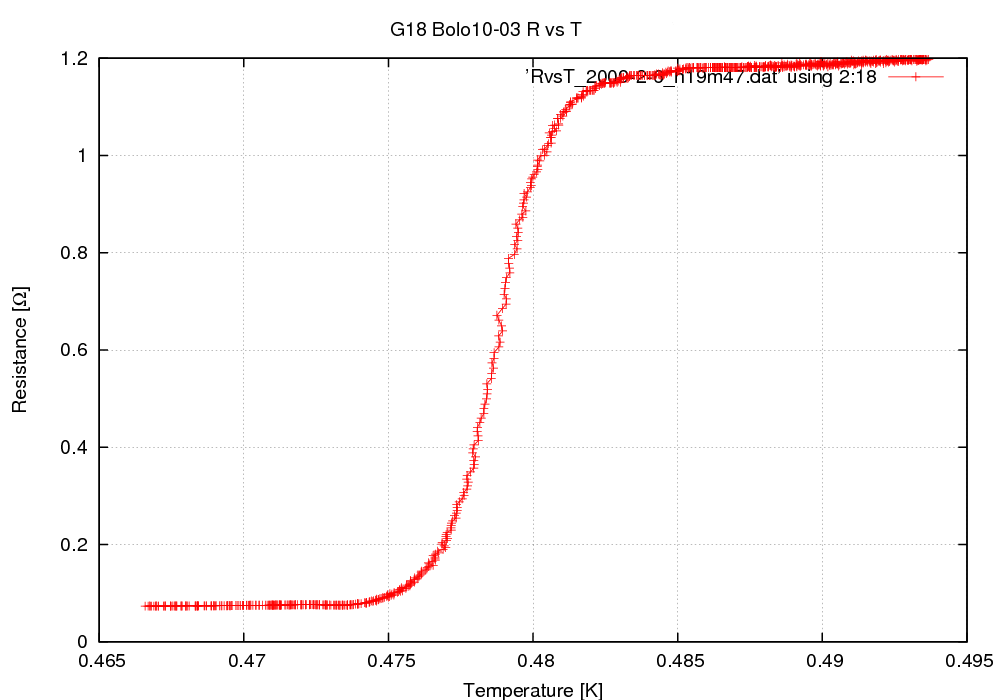
\includegraphics[height=2.5in]{figures/G18_bolo10-03_RvsT_oral}
\caption{Resistance versus temperature for an \ac{EBEX} bolometer.
\label{fig:r_vs_t} }
\end{center}
\end{figure}



\textcolor{red}{Four noise sources, fundamental limit set by photon arrival stats}

1. Electronic/Readout

2. Johnson

3. Phonon (ballistic vs �?)

4. Photon (a. Poisson process, b. Shot noise)



The sensitivity of the instrument is quantified by the \ac{NEP}. 
\ac{NEP} is defined as the absorbed power required to produce a signal-to-noise ratio of one in an electrical bandwidth of one~Hz. 
%not important?
%Note, sometimes \ac{NEP} is instead defined as the \textit{incident} power required to produce a signal-to-noise ratio of one in an electrical bandwidth of one~Hz, \textcolor{red}{cite who??}.
The predicted detector \ac{NEP}, $N$, is given by 
\begin{equation}
N^{2} = N_{photon}^2 + N_{phonon}^2 + \frac{1}{S_I^2} ( N_{Johnson}^2 + N_{readout}^2 )
\end{equation}
\begin{equation}
= 2h\nu P_{rad} + \xi \frac{P_{rad}^2}{\Delta \nu} + \gamma 4k_{B} T^2 G + \frac{1}{S_I^2} (\frac{4k_BT}{R} + N_{readout}^2 )
\label{eq:nep}
\end{equation}
where $h$ is Planck's constant, $\nu$ is the center of the observation frequency band, $P_{rad}$ is the radiative power absorbed by the bolometer, $\xi$ is a unitless number between zero and one quantifying the contribution of photon correlation noise, $\Delta \nu$ is the width of the observation frequency band, $\gamma$ is a unitless number between zero and one accounting for the temperature gradient along the link from the \ac{TES} to the bath, $k_{B}$ is Boltzmann's constant, $T$ is the \ac{TES} temperature, $G$ is the bolometer dynamic thermal conductance, $S_{I}$ is the bolometer current responsivity, and $R$ is the \ac{TES} resistance~\citep{Mather1982a}. 



%%%%%%%%%%%%%%%%%%%%%%%%%%%%%%%%%%%%%%%%%%%%%%%%%%%%%%%%%%%%%%%%%%%%%%%%%%%%%}}}



%%%%%%%%%%%%%%%%%%%%%%%%%%%%%%%%%%%%%%%%%%%%%%%%%%%%%%%%%%%%%%%%%%%%%%%%%%%%%%%%
% Detector Design Modifications for Space-Like Environment {{{
%%%%%%%%%%%%%%%%%%%%%%%%%%%%%%%%%%%%%%%%%%%%%%%%%%%%%%%%%%%%%%%%%%%%%%%%%%%%%%%%
\section{Detector Design}
\label{sec:detector_design}
%%%%%%%%%%%%%%%%%%%%%%%%%%%%%%%%%%%%%%%%%%%%%%%%%%%%%%%%%%%%%%%%%%%%%%%%%%%%%%%%

Discuss target detector parameters. Be very clear about which changes were made to fabrication process in order to optimize the detector sensitivity for a space-like environment and for EBEX.

1. Ideal normal resistance.  
The target normal resistance for all bands was 1.5~$\Omega$ in order to ensure the detector, when biased in the transition, remained in the stable regime where the detector electrical bandwidth, determined in part by the resistance, exceeded the \ac{TES} thermal bandwidth by at least XXX (CITE PAPER). THIS HAS NOTHING TO DO WITH A SPACE-LIKE ENVIRONMENT.

2. Ideal transition temperature for our bath temperature. NEED: PLOT OF PHONON NOISE AS FUNCTION OF TRANSITION TEMPERATURE (GIVEN A FIXED EBEX BATH TEMPERATURE OF 260 MK)

3. Ideal thermal conductance and heat capacity of TES/web 
\begin{itemize}
\item When we set our target $G$, we included a safety factor of 2.5 times the expected load from the \ac{CMB} in case of excess load or fluctuations or other shit. 
\end{itemize}


4. Ideal time constant


The \ac{TES} is a square of 19 x 19~$\mu m^{2}$.

\begin{figure}[ht!]
\begin{center}
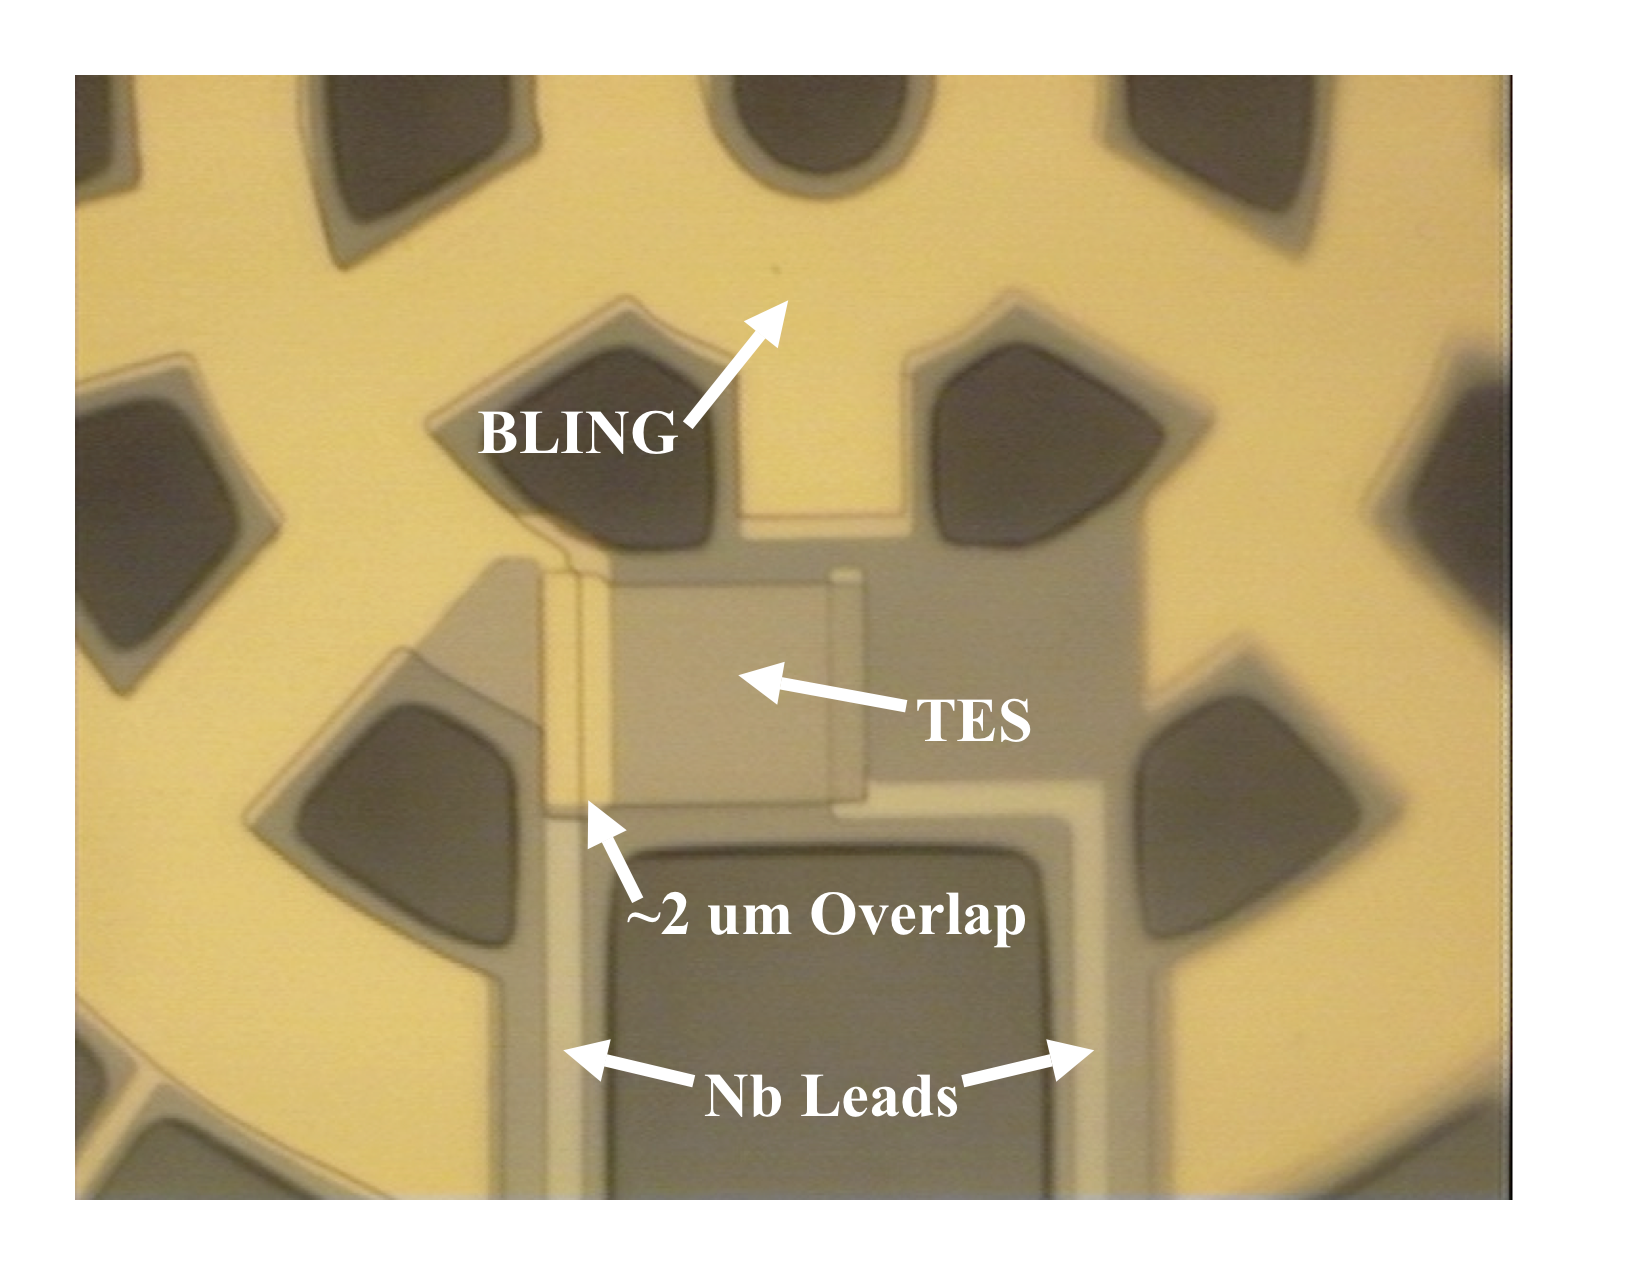
\includegraphics[height=2.5in]{figures/EBEX_BLINGTES_Annotated.png}
\caption{\ac{EBEX} bling and \ac{TES}. Figure courtesy of Benjamin Westbrook. \textcolor{red}{How do I say this is Ben's not mine??}
\label{fig:bling_and_tes} }
\end{center}
\end{figure}

\emph{We wanted to decrease G, so we roughly doubled the leg length (where you could find space). Do you have pictures of the mask with the original leg length and the final leg length?
For 150, we pulled out all of the stops we could.  We doubled the length of 7/8 legs from 0.5mm to 1.05 mm. For the 8th leg, we increased it's length by a factor of 3 to 1.45 mm. In addition, we made all the legs expect the one with Nb 6 um wide.  The old design had 2 / 8 with 17 um wide legs. 
We wanted to decrease Tc, so you messed around with the thickness of the Al layer in our Al/Ti TES sandwich. 
Specifically we modulate the thickness of the Al (30-50 nm) compared to the Ti layer, which we held at constant thickness (~110nm). More Al means higher Tc and lower Rn (and converse is true).  Technically it's not a sandwhich (that's Shaul's term) it's just a bilayer, Al with Ti on top. Not Al-Ti-Al nor Ti-Al-Ti.
We wanted to keep the time constant (C/G) the same, so we decreased the heat capacitance by decreasing the thickness of the bling (or we did something else??). 
So we still had a BLING layer (the waffle pattern at the center of the photos).  However, we didn't add any EXTRA gold here like SPT and APEX had.  The C of the EBEX detectors comes from 20 nm of Gold on a 1um thick layer of Silicon nitride.  Where as the SPT/APEX had the 20nm of gold for the web, the 1 um of Silicon Nitrides, + ~500-700 nm of extra BLING only gold at the center.  Since gold has a large heat capacity, it dominates the total C in the detectors.  I attached a quick memo on this I wrote for Shaul that summarized the changes in heat capacity. 
Why did we move away from the circle bling design? 
This is because the waffle pattern has a lower G than the circle so that heat absorbed by the web more efficiently couples to the TES, which ultimately increases optical efficiency (and thus sensitivity) as the TES has time to sense it (i.e it thermalizes) before the heat is dissipated to the bath via the legs.}




\begin{table}[ht!]
\centering
%\footnotesize
\begin{tabular}{| c | c c | c c | c c |}\hline
\multicolumn{1}{|c}{Band (GHz)}   &  \multicolumn{2}{|c}{150}   & \multicolumn{2}{|c}{250}   & \multicolumn{2}{|c|}{410}  \\% \hline
                                     & Design & Measured & Design & Measured & Design & Measured  \\ \hline
$R_{n}$ ($\Omega$)            & 1.5  & 1.9  & 1.5  & 1.5  & 1.5  & 1.4  \\
$T_{c}$ (K)                        & 0.44 & 0.45 & 0.44 & 0.49 & 0.44 & 0.47  \\
$\overline{G}$ (pW/K)       & 30   & 39 & 40   & 53 & 50   & 63  \\
$\tau_{0}$ (ms)                 & 17 & 88$^\dagger$  & 13  &  46$^\dagger$  &  10 &  57$^\dagger$  \\
$C$ (pJ/K)*                         & 0.5  & 3.8$^\dagger$ & 0.5  & 3.3$^\dagger$  & 0.5   & 8.4$^\dagger$  \\ \hline
 Wafer Thickness ($\mu$m)   & \multicolumn{2}{|c|}{150}  & \multicolumn{2}{|c|}{90}  & \multicolumn{2}{|c|}{56}  \\
$\alpha$ (mm)                &  \multicolumn{2}{|c|}{1.05}   & \multicolumn{2}{|c|}{1.0}   &  \multicolumn{2}{|c|}{0.5}  \\
$\beta$ (mm)                & \multicolumn{2}{|c|}{1.45} & \multicolumn{2}{|c|}{1.0}  & \multicolumn{2}{|c|}{0.5}  \\ \hline
\multicolumn{7}{l}{\footnotesize$^\dagger$ Median of measurements on a single wafer at each frequency; see Section~\ref{sec:time_constants}.}\\
\multicolumn{7}{l}{\footnotesize* Calculated from time constant and thermal conductivity.}
\end{tabular}
\caption{STOLE THIS TABLE FROM THE PAPER FOR NOW. WANT SOMETHING SIMILAR HERE. Designed and measured detector parameters for each of the frequency
bands.  The values in the `measured' columns are median values for 
all detectors on wafers used for flight.  Description of the measurements and histograms and further discussion 
of the measured values are given in Section \ref{sec:detector_characterization}.
For the parameters $\alpha$ and $\beta$, shown in Figure~\ref{fig:Bolometer_Overview} we give the design values. 
The lithography was generally accurate to within 0.5~$\mu$m.
\label{tab:Design_Params} }
\end{table}


%%%%%%%%%%%%%%%%%%%%%%%%%%%%%%%%%%%%%%%%%%%%%%%%%%%%%%%%%%%%%%%%%%%%%%%%%%%%%}}}